% =====================================================================
%  Entity-Level Sentiment from Financial News -- project report
%
%  Build (from the docs/ directory, three passes for cross-references):
%      pdflatex project_report.tex
%  Figures are read from the repository via \graphicspath{{../}}; the two prompt
%  listings in Appendix A come from docs/report_assets/ (ASCII copies of the
%  files in data_label_criteria/).  Needs only packages shipped with a basic
%  TeX Live (2015 or later).
% =====================================================================
\documentclass[11pt,letterpaper]{article}

\usepackage[T1]{fontenc}
\usepackage[utf8]{inputenc}
\usepackage{lmodern}
\usepackage{microtype}
\usepackage[margin=1in]{geometry}
\usepackage{amsmath,amssymb,bm,mathtools}
\usepackage{booktabs,array,tabularx,multirow}
\usepackage{xcolor,colortbl}
\usepackage{graphicx,float}
\usepackage{caption,subcaption}
\usepackage{parskip}
\usepackage{listings}
\usepackage{tikz}
\usetikzlibrary{arrows,positioning,fit,calc,backgrounds,shapes.geometric,decorations.pathreplacing}
\usepackage[colorlinks=true,linkcolor=blue!55!black,citecolor=blue!55!black,urlcolor=blue!55!black]{hyperref}
\graphicspath{{../}}

\captionsetup{font=small,labelfont=bf,skip=6pt,justification=raggedright,singlelinecheck=true}
\setlength{\emergencystretch}{2em}
\newcolumntype{Y}{>{\raggedright\arraybackslash}X}
\newcolumntype{R}{>{\raggedleft\arraybackslash}X}
\newcolumntype{P}[1]{>{\raggedright\arraybackslash}p{#1}}
\setcounter{tocdepth}{1}
\lstset{basicstyle=\ttfamily\footnotesize,columns=fullflexible,keepspaces=true,
        frame=lines,framesep=5pt,xleftmargin=4pt,breaklines=true}

% ---------- colours ----------
\definecolor{encblue}{RGB}{222,235,247}
\definecolor{encblueD}{RGB}{49,99,160}
\definecolor{nergreen}{RGB}{226,240,217}
\definecolor{nergreenD}{RGB}{56,118,29}
\definecolor{sentorange}{RGB}{252,228,214}
\definecolor{sentorangeD}{RGB}{197,90,17}
\definecolor{maskgray}{RGB}{238,238,238}
\definecolor{maskgrayD}{RGB}{95,95,95}
\definecolor{ioyellow}{RGB}{255,243,205}
\definecolor{rowgray}{gray}{0.94}

% ---------- tikz styles ----------
\tikzset{
  blk/.style={draw,rounded corners=3pt,align=center,inner sep=5pt,
              minimum height=2.3em,font=\small,line width=0.6pt},
  enc/.style={blk,fill=encblue,draw=encblueD},
  ner/.style={blk,fill=nergreen,draw=nergreenD},
  sen/.style={blk,fill=sentorange,draw=sentorangeD},
  msk/.style={blk,fill=maskgray,draw=maskgrayD,dashed},
  io/.style={blk,fill=ioyellow,draw=black!60},
  arr/.style={-latex',line width=0.7pt},
  darr/.style={-latex',line width=0.7pt,dashed,draw=maskgrayD},
  lbl/.style={font=\scriptsize,fill=white,inner sep=1.5pt,text=black!70},
}

\newcommand{\code}[1]{\texttt{#1}}
\newcommand{\mH}{\bm{H}}
\newcommand{\vm}{\bm{m}}
\newcommand{\vg}{\bm{g}}
\newcommand{\R}{\mathbb{R}}
\newcommand{\bps}{\,bps}

\title{\textbf{Entity-Level Sentiment from Financial News}\\[4pt]
  \large Model, training, validation, and tests against S\&P~500 returns and volatility}
\author{Russell Ding\thanks{Independent project, built on the author's own time, hardware and data
  subscription; no employer code or data is involved. The code and analyses were produced with
  Claude Code under the author's direction and were reviewed read-only by two other model-based
  reviewers (Codex and Kimi); all conclusions were verified by the author. Code and this report:
  \url{https://github.com/Russell-Ding/entity_sentiment_model_pipeline}.}}
\date{September 2026}

\begin{document}
\maketitle

\begin{abstract}
\noindent
This report summarises a two-part project. The first part is a model that reads a complete
financial news article and assigns every company, ticker, person and organisation it finds a
sentiment score in $(-0.95, 0.95)$ that expresses the \emph{implication of the news for that
entity}, not the tone of the article. It is a shared Longformer-large encoder (2{,}048 tokens per
article) with a CRF-decoded entity tagger and a cross-attention sentiment head, 439M parameters in
total, trained by distillation from LLM-generated labels: three stages on about 20{,}000
articles, then a head-only retrain on about 30{,}000 relabelled articles with a
concordance-based loss. On a held-out test split the
sentiment scores reach a Pearson correlation of 0.64 with the labels and match their spread; the
entity tagger, which has to find the entities before they can be scored, is the bottleneck at
about 48\% coverage. The second part scores 118{,}033 wire-grade articles about 502 S\&P~500
constituents (2020--2025) and tests whether the scores predict returns. They do not: the
apparently strong first-pass evidence (one-day rank IC $+0.020$, Newey--West $t$ 3.7; a
close-entry long-short Sharpe of 2.9) was look-ahead, because about a quarter of the articles,
including the after-hours earnings spike, had been dated to a session whose close preceded their
publication. Rebuilt with a 15:45~ET knowability cutoff, the IC is indistinguishable from zero
at every horizon and every daily-bar execution tested loses money. Two results survive: the
scores align strongly with the contemporaneous overnight reaction, which makes the model a
useful measurement instrument, and the \emph{magnitude} of sentiment predicts next-day absolute
returns beyond trailing realised volatility (rank IC $+0.024$, $t$ 5.3).
\end{abstract}

\tableofcontents

% =====================================================================
\section{Summary of findings}
\label{sec:summary}

The project asked five questions. Table~\ref{tab:glance} gives the short answers; the rest of the
report gives the evidence. Sections~\ref{sec:data}--\ref{sec:validation} cover the model and
Section~\ref{sec:signal} the market tests; Appendix~\ref{app:prompts} reproduces the labelling
prompts and Appendix~\ref{app:repo} lists what the public repository contains.

\begin{table}[H]
\centering\small
\begin{tabularx}{\linewidth}{@{}P{4.1cm}P{2.6cm}Y@{}}
\toprule
\textbf{Question} & \textbf{Answer} & \textbf{Evidence} \\
\midrule
Can a long-document model score sentiment per entity? & Yes, moderately well &
  v2.1 held-out test: Pearson 0.64, concordance 0.64, prediction spread equal to the labels';
  95\% of entities within one sentiment bucket of the label; strongest on tickers ($r$ 0.81). \\
\rowcolor{rowgray}
Does the end-to-end pipeline find the entities? & Only about half &
  Entity coverage 42--48\%; span precision 0.86 but recall 0.47 on sentiment-bearing types. \\
Do the scores predict next-day returns? & No detected edge &
  Knowability-corrected one-day rank IC $-0.007$ ($t$ $-1.4$); the implementable market-on-close
  strategy has gross Sharpe $-0.55$; next-open entry is negative at every holding period tested.
  One channel, pre-market news at the same day's open, remains untested. \\
\rowcolor{rowgray}
Do the scores explain the market's reaction? & Yes &
  First-pass day-one quintile spread $+36\bps$, of which $+41\bps$ is the overnight gap after
  publication and $-5\bps$ the tradable intraday part. \\
Does sentiment predict volatility? & Yes, modestly &
  $|$sentiment$|$ vs.\ next-day $|$return$|$ after trailing realised volatility: rank IC $+0.024$
  ($t$ 5.3); $+0.019$ ($t$ 3.7) with an extra same-day $|$return$|$ control (independent
  replication). Not yet hardened or reproducible from a committed script. \\
\bottomrule
\end{tabularx}
\caption{The project at a glance. IC = information coefficient (daily cross-sectional Spearman
correlation), $t$ = Newey--West $t$-statistic, bps = basis points.}
\label{tab:glance}
\end{table}

\textbf{Two provenance notes.} First, the market tests were run on scores produced by the v2.0
checkpoint, not v2.1 as the study's working documents state: the inference files predate the v2.1
release, the inference launcher hard-codes the v2.0 checkpoint, and re-scoring stored articles
reproduces the saved values only with v2.0. The corrected attribution is used throughout this
report, and a correction note has been added to the study documents. Second, everything here was
built with model-based tooling; the first-pass conclusion of the market study was wrong, and the
correction is reported in full because the correction is the substantive result.

% =====================================================================
\section{Data and labels}
\label{sec:data}

\subsection{News corpus}

The corpus is the EODHD news feed for the S\&P~500 universe: 1.69 million articles from 2020 to
2025, stored per primary ticker with a publication timestamp, source and URL. Every article was
assigned a \emph{source tier} and a content type by a rule set distilled from a 5{,}000-article
LLM-labelled sample: tier~1 is wire-grade reporting (Reuters, Bloomberg, AP, WSJ and similar, 9.6\% of the
corpus), tier~2 is secondary and analytical press including market wraps, analyst-call pieces and
earnings transcripts (9.0\%), and tier~3 is algorithmic and search-optimised bulletins,
syndicated press releases and listicles (81.3\%). The tiers were designed to carry a
per-article loss weight; in the released training path they select which articles enter the
training subsets rather than reweighting the loss. The market study used tier-1 articles only.

Coverage is uneven, and this matters downstream. The feed carries no Bloomberg or AP content for
November--December 2024 (a provider-side outage, confirmed by inspecting the raw feed), and it
has no tier-1 coverage of NVIDIA's earnings week of 23--29 May 2023. A coverage-gap flag was
added to the daily series so that readings following a blackout can be identified. One wire
service contributes about 14{,}500 tier-1 items that turned out to be 300-character paywall
stubs; they were marked for demotion to tier~2 but the corpus was never re-tiered, so they are
filtered by the per-ticker daily aggregation and \emph{not} by the 502-name signal panel of
Section~\ref{sec:signal}, which reads the inference files directly. The news and price data are
not redistributed (EODHD terms).

\subsection{Labels by distillation}

No human-annotated corpus exists for entity-level financial sentiment at this granularity, so
labels were generated by large language models from a written specification and then filtered.
Three label sets were produced over the life of the project (Table~\ref{tab:labels}); the model
versions in Section~\ref{sec:training} map onto them one to one.

\begin{table}[H]
\centering\small
\begin{tabularx}{\linewidth}{@{}P{2.5cm}P{3.0cm}YP{3.4cm}@{}}
\toprule
\textbf{Label set} & \textbf{Labeller} & \textbf{Size and splits} & \textbf{Used for} \\
\midrule
v1 (Jan 2026) & Claude Haiku~4.5 & 2{,}133 train / 235 validation articles; COMPANY entities only &
  v1.0 model (Longformer-base) \\
\rowcolor{rowgray}
Sonnet relabels (Feb--Apr 2026) & Claude Sonnet, simplified prompt &
  17{,}587 train / 2{,}130 validation; evaluation holdouts of 6{,}750 relabelled and 9{,}371
  original-label articles, drawn from non-overlapping sources &
  v2.0 model, all three training stages \\
Decisive set (Jun 2026) & DeepSeek v4-flash with the \emph{decisive} prompt; PERSON entities
  re-scored by Kimi &
  30{,}131 tier-1 articles after near-duplicate removal, split by article id into 27{,}015 /
  1{,}558 / 1{,}558 (train / validation / test) &
  v2.1 head retrain and its in-distribution evaluation; the Sonnet holdout is kept for the
  tagging and cross-distribution checks \\
\bottomrule
\end{tabularx}
\caption{Label sets. The two prompts used for the decisive set are reproduced in
Appendix~\ref{app:prompts}.}
\label{tab:labels}
\end{table}

Each labelled article carries a list of entity records. A record has a canonical id and name, a
type (ORG, TICKER, PERSON, MONEY, PERCENT, DATE), the literal name mentions in the text, the
coreferent mentions (\emph{it}, \emph{the company}, \emph{the iPhone maker}) kept separately, and
a sentiment score in $[-1, 1]$ for ORG, TICKER and PERSON records; MONEY, PERCENT and DATE
records are extracted but carry no score. A company and its ticker symbol, when both appear
literally, are separate records that share one score. Mentions are given as strings and located
in the text afterwards by code, which removed the character-offset errors that plagued the first
label set.

\subsection{What the score means}

The scoring rule is the part of the specification that changed most between label sets, and it
is the reason v2.1 exists. The Sonnet prompt asked for the \emph{tone} of the article with respect
to the entity, and 0.0 for ``factual mention''. Financial news is written in a flat, factual
register, so that rule produced a label distribution heavy in zeros and a model that hedged
toward zero. The decisive prompt scores the \emph{implication} of the news for the entity even
when it is reported neutrally (a lawsuit defendant is negative; an earnings beat is positive)
and reserves 0.0 for entities with no stake in the story (an analyst's employer cited for a
rating, a data source, an exchange). Table~\ref{tab:bands} gives the bands. About 59\% of the
scored entities in the decisive set are still incidental, which shapes the loss design in
Section~\ref{sec:loss}.

\begin{table}[H]
\centering\small
\begin{tabularx}{\linewidth}{@{}llY@{}}
\toprule
\textbf{Score} & \textbf{Meaning} & \textbf{Typical trigger} \\
\midrule
$-1.0$ to $-0.7$ & very negative & bankruptcy, fraud, criminal charges \\
$-0.6$ to $-0.4$ & moderately negative & lawsuit or antitrust defendant, earnings miss, downgrade, layoffs, recall, probe \\
$-0.3$ to $-0.1$ & slightly negative & cautious outlook, minor headwind, lagging a rival \\
$0.0$ & neutral & incidental, no-stake mention only \\
$+0.1$ to $+0.3$ & slightly positive & minor beat, modest gain, favourable mention \\
$+0.4$ to $+0.6$ & moderately positive & earnings beat, upgrade, major deal or launch, winning a suit \\
$+0.7$ to $+1.0$ & very positive & record results, blockbuster product, transformative win \\
\bottomrule
\end{tabularx}
\caption{Sentiment bands in the decisive labelling prompt (Appendix~\ref{app:prompts}).}
\label{tab:bands}
\end{table}

\subsection{Quality controls}

Near-duplicate articles (wire re-runs with distinct ids) were removed before splitting, and the
splits are disjoint by article id. An automated quality guardian sampled the completed labels
during each run and halted it when format, extraction, neutrality or failure rates breached a
threshold.

PERSON scores from the first DeepSeek pass were noticeably worse than ORG scores, so PERSON
entities were re-scored with a dedicated prompt wherever the request was accepted; cases the
re-scoring model declined kept their original score. Measured afterwards with the
\emph{unchanged} v2.0 model, the re-scored entities correlate with their labels at 0.50 and the
1{,}334 that were not re-scored at 0.29. These are different subsets rather than a before-and-after
measurement of the same cases, so the comparison suggests that the re-score fixed labels rather
than fitting the model, without establishing it.

After the v2.1 retrain, the highest-confidence disagreements between model and label were
extracted for manual adjudication. The v2.1 model card records the outcome as about one clear
label error in roughly 24 adjudicated cases, which is the basis for treating the retrain gains
as real rather than fitted noise; the released audit file lists the cases and the disagreement
rates but not the adjudications themselves.

% =====================================================================
\section{Model}
\label{sec:model}

Figure~\ref{fig:overview} shows the model. One shared encoder produces contextual token states;
two small heads read them. The heads are coupled through two masks that carry entity positions:
the \emph{entity masks} select which token states become the queries of the sentiment head, and
the \emph{global-attention mask} tells the encoder itself which tokens may attend to the whole
document. During training the masks come from the gold entity mentions; at inference they come
from the tagger's predicted spans, so the encoder is run twice per article.

\begin{figure}[!t]
\centering
\resizebox{\linewidth}{!}{%
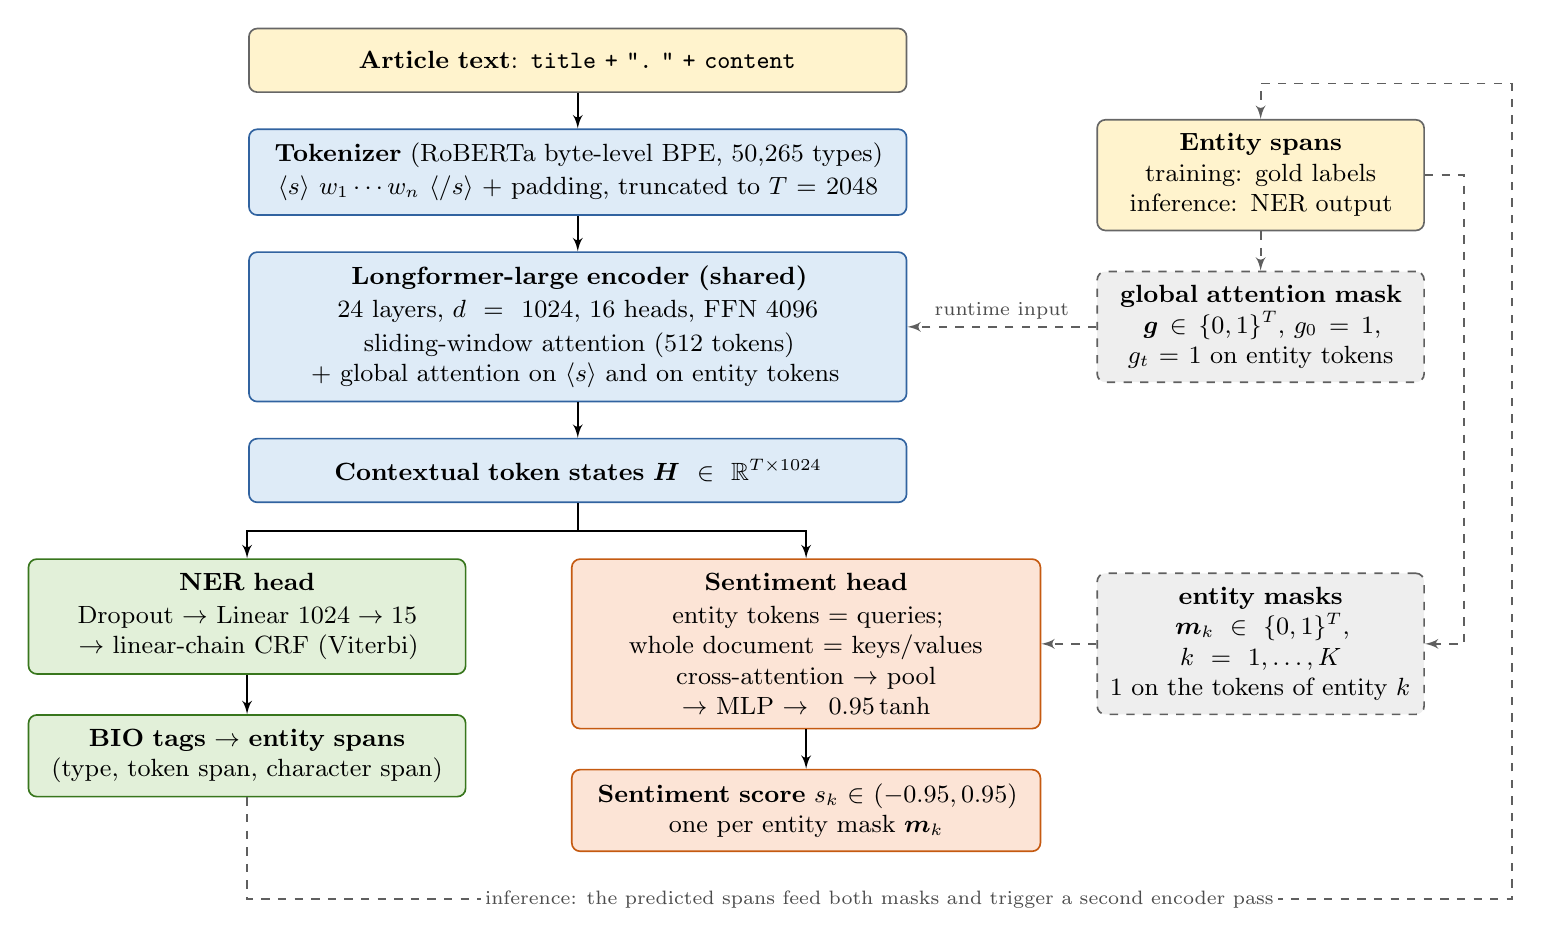
\begin{tikzpicture}[x=1cm,y=1cm]
\node[io,text width=8cm] (text) at (0,0)
  {\textbf{Article text}: \code{title + ".\ " + content}};
\node[enc,text width=8cm,anchor=north] (tok) at ($(text.south)+(0,-0.45)$)
  {\textbf{Tokenizer} (RoBERTa byte-level BPE, 50{,}265 types)\\[1pt]
   $\langle s\rangle\; w_1 \cdots w_n\; \langle/s\rangle$ + padding, truncated to $T=2048$};
\node[enc,text width=8cm,anchor=north] (encoder) at ($(tok.south)+(0,-0.45)$)
  {\textbf{Longformer-large encoder (shared)}\\[1pt]
   24 layers, $d=1024$, 16 heads, FFN 4096\\[1pt]
   sliding-window attention (512 tokens)\\ + global attention on $\langle s\rangle$ and on entity tokens};
\node[enc,text width=8cm,anchor=north] (H) at ($(encoder.south)+(0,-0.45)$)
  {\textbf{Contextual token states} $\mH\in\R^{T\times 1024}$};
\node[ner,text width=5.2cm,anchor=north] (nerhead) at ($(H.south)+(-4.2,-0.7)$)
  {\textbf{NER head}\\[1pt] Dropout $\to$ Linear $1024\!\to\!15$\\ $\to$ linear-chain CRF (Viterbi)};
\node[sen,text width=5.6cm,anchor=north] (senthead) at ($(H.south)+(2.9,-0.7)$)
  {\textbf{Sentiment head}\\[1pt] entity tokens = queries;\\ whole document = keys/values\\
   cross-attention $\to$ pool $\to$ MLP $\to 0.95\tanh$};
\node[ner,text width=5.2cm,anchor=north] (spans) at ($(nerhead.south)+(0,-0.5)$)
  {\textbf{BIO tags $\to$ entity spans}\\ (type, token span, character span)};
\node[sen,text width=5.6cm,anchor=north] (score) at ($(senthead.south)+(0,-0.5)$)
  {\textbf{Sentiment score} $s_k\in(-0.95,0.95)$\\ one per entity mask $\vm_k$};
\node[msk,text width=3.8cm,anchor=west] (gmask) at ($(encoder.east)+(2.4,0)$)
  {\textbf{global attention mask}\\ $\vg\in\{0,1\}^T$, $g_0=1$,\\ $g_t=1$ on entity tokens};
\node[io,text width=3.8cm,anchor=south] (hub) at ($(gmask.north)+(0,0.5)$)
  {\textbf{Entity spans}\\ training: gold labels\\ inference: NER output};
\node[msk,text width=3.8cm,anchor=west] (emask) at (gmask.west |- senthead.east)
  {\textbf{entity masks}\\ $\vm_k\in\{0,1\}^T$, $k=1,\dots,K$\\ 1 on the tokens of entity $k$};
\draw[arr] (text) -- (tok);
\draw[arr] (tok) -- (encoder);
\draw[arr] (encoder) -- (H);
\draw[arr] (H.south) -- ++(0,-0.35) -| (nerhead.north);
\draw[arr] (H.south) -- ++(0,-0.35) -| (senthead.north);
\draw[arr] (nerhead) -- (spans);
\draw[arr] (senthead) -- (score);
\draw[darr] (hub) -- (gmask);
\draw[darr] (hub.east) -- ++(0.5,0) |- (emask.east);
\draw[darr] (gmask.west) -- (encoder.east) node[lbl,midway,above=1pt] {runtime input};
\draw[darr] (emask.west) -- (senthead.east);
\coordinate (bl) at ($(spans.south |- score.south)+(0,-0.6)$);
\coordinate (br) at ($(emask.east)+(1.1,0)$);
\coordinate (tr) at ($(hub.north)+(0,0.45)$);
\draw[darr] (spans.south) -- (bl) -- (bl -| br) -- (br |- tr) -- (tr) -- (hub.north);
\node[lbl] at ($(bl)!0.5!(bl -| br)$)
  {inference: the predicted spans feed both masks and trigger a second encoder pass};
\end{tikzpicture}}
\caption{Model structure. Solid arrows are the forward tensor flow; dashed arrows carry the two
masks through which entity positions enter the network, and the inference feedback path that
rebuilds those masks from the predicted spans.}
\label{fig:overview}
\end{figure}

\textbf{Encoder.} \code{allenai/longformer-large-4096} \cite{beltagy2020longformer}: 24 layers,
hidden size 1{,}024, 16 heads, a 512-token sliding attention window plus global attention on
selected tokens. Articles are truncated or padded to exactly 2{,}048 tokens, half of the
encoder's 4{,}096-position capacity; the budget was chosen for GPU memory and throughput, and
longer articles lose their tail. Longformer was chosen over 512-token encoders because the sentence that settles an
entity's sentiment is often far from its mention, and the global-attention mechanism gives a
natural way to make the encoder \emph{entity-aware}: every token can attend to the entity tokens
and the entity tokens can attend to the whole article.

\textbf{NER head.} Dropout, a linear layer to 15 BIO tags (\emph{O} plus begin/inside tags for
COMPANY, TICKER, PERSON, ORG, MONEY, PERCENT and DATE; the COMPANY tag is a legacy of the first
label set and unused by v2 labels, which file companies under ORG) and a linear-chain CRF decoded
by Viterbi. Tags are converted to spans with a lenient decoder that repairs an \emph{inside} tag
without a preceding \emph{begin}. In the released v2 weights the CRF transition scores never
moved from their initial values (Section~\ref{sec:crf}), so the tagger behaves as a per-token
classifier followed by span repair.

\textbf{Sentiment head.} For each entity mask, the entity's token states become queries and the
whole document's states become keys and values of an 8-head cross-attention (with layer
normalisation on both sides and a residual connection); the attended entity tokens are mean-pooled,
normalised, and mapped by a three-layer MLP ($1024\to512\to128\to1$, GELU, dropout) to a scalar
that is squashed as $s = 0.95\tanh(z)$. The head has 4.80M parameters. All entities of an
article are scored in one call, so an article with $K$ entities costs one encoder pass plus one
batched head evaluation.

\textbf{Inference: two encoder passes.} Pass~1 runs the encoder with global attention on the
$\langle s\rangle$ token only and decodes entity spans. Pass~2 runs it again with global attention
on $\langle s\rangle$ plus every predicted sentiment-bearing span and scores each span. Spans with
the same surface text and type are averaged into one record per entity per article; MONEY,
PERCENT and DATE spans are dropped. Making a single encoder serve both regimes is what the
training procedure has to solve (Section~\ref{sec:training}).

\begin{table}[H]
\centering\small
\begin{tabular}{@{}lrl@{}}
\toprule
\textbf{Component} & \textbf{Parameters} & \textbf{Trained in} \\
\midrule
Longformer-large encoder & 434{,}600{,}960 & Stages 1--2 (frozen afterwards) \\
NER head (linear + CRF) & 15{,}630 & Stages 1--2 (frozen afterwards) \\
Sentiment head (cross-attention + MLP) & 4{,}795{,}137 & Stage 3; retrained for v2.1 \\
\midrule
Total & 439{,}411{,}727 & \\
\bottomrule
\end{tabular}
\caption{Parameter budget of the v2.x model (read from the checkpoint).}
\label{tab:params}
\end{table}

% =====================================================================
\section{Training procedure}
\label{sec:training}

\subsection{Why the recipe has stages}

An earlier version of the model was trained end to end with global attention always placed on the
gold entity tokens. With gold entity positions it tagged well (F1 0.74), but in real use there are
no gold positions: the tagger must run with global attention on $\langle s\rangle$ alone, a regime
the encoder had never seen, and end-to-end F1 collapsed to 0.05. The fix, \emph{global-attention
dropout}, hides the entity-aware global attention for a random 30\% of training samples so that
the encoder learns to produce useful states in both regimes. Around that idea the recipe became
three stages that train progressively fewer parameters, followed by a head-only retrain when the
labels changed (Table~\ref{tab:stages}).

\begin{table}[!t]
\centering\footnotesize
\begin{tabularx}{\linewidth}{@{}P{1.9cm}P{2.5cm}P{2.5cm}YP{3.3cm}@{}}
\toprule
\textbf{Stage} & \textbf{Trains} & \textbf{Data} & \textbf{Loss and settings} & \textbf{Outcome} \\
\midrule
1. NER & encoder + NER head (all parameters) & Sonnet relabels: 17{,}587 train / 2{,}130 val &
  CRF negative log-likelihood only (sentiment weight 0). 5 epochs, batch 24, AdamW, LR $2{\times}10^{-5}$,
  mixed precision, gradient checkpointing; global-attention dropout $p=0.3$, ramped up over the
  first 30\% of steps &
  Best CLS-only NER F1 0.584 at epoch 2 (entity-aware F1 about 0.76); this checkpoint feeds Stage 3 \\
\rowcolor{rowgray}
2. Joint & everything & same &
  CRF loss + sentiment loss with a curriculum: NER weight $1.0\to0.5$, sentiment weight
  $0.3\to1.0$. 5 epochs, batch 24, LR $10^{-5}$, dropout $p=0.3$ without ramp &
  Joint training pulled the encoder away from the CLS-only optimum (CLS-only F1 to 0.53); its
  checkpoint was therefore not used downstream \\
3. Sentiment & sentiment head only (freshly initialised); encoder and NER head frozen, loaded from
  the Stage-1 checkpoint & same &
  $0.5\,\mathrm{MSE} + 0.5\,(1-\rho)$ with $\rho$ the batch Pearson correlation
  (Eq.~\ref{eq:legacy}). 10 epochs, batch 80, LR $5{\times}10^{-4}$, no attention dropout &
  Best epoch 9: validation $r$ 0.511. Packaged as \textbf{v2.0} (17 May 2026) \\
\rowcolor{rowgray}
v2.1 head retrain & sentiment head only, initialised from the v2.0 head; encoder and NER head frozen &
  Decisive set: 27{,}015 / 1{,}558 / 1{,}558 &
  weighted Huber + $(1-\mathrm{CCC})$ + sign penalty (Eq.~\ref{eq:ccchuber}). 10 epochs, batch 48,
  head LR $5{\times}10^{-4}$, cosine schedule, best epoch by validation CCC &
  Best epoch 10: validation CCC 0.618. Packaged as \textbf{v2.1} (20 June 2026); encoder and NER
  head byte-identical to v2.0 \\
\bottomrule
\end{tabularx}
\caption{The training sequence. The documented Colab recipe uses a single high-memory GPU and
estimates roughly 14 hours for Stages 1--3 together; per-run hardware and timing logs are not
part of the release.}
\label{tab:stages}
\end{table}

Two details of the sequence are easy to miss. Stage~3 loads the \emph{Stage-1} checkpoint, not
Stage~2's, because Stage~3 discards whatever sentiment head it inherits and only needs the best
encoder for the CLS-only tagging regime. And the v2.1 head was \emph{warm-started} from the v2.0
head rather than re-initialised: the retrain script loads the full v2.0 state and never resets
the head, and the run ledger's pre-training baseline for the sibling arm is the v2.0 head's own
validation score. (An earlier version of the v2.1 model card described the head as
re-initialised; the card's corrections section now fixes this.)

\subsection{Loss functions}
\label{sec:loss}

Sentiment is a regression on the scored entities of a batch. The v2.0 head used
\begin{equation}
\label{eq:legacy}
L_{\text{v2.0}} = \tfrac12\,\mathrm{MSE}(\hat y, y) + \tfrac12\,\bigl(1-\rho(\hat y, y)\bigr),
\end{equation}
which has a specific weakness. On a label distribution that is 59\% zeros, mean-squared error is
minimised by shrinking uncertain predictions toward zero, and the Pearson term is
scale-invariant, so it cannot see the shrinkage: a model that predicts exactly half the true
magnitude has $\rho = 1$. The trained v2.0 head accordingly predicted with 57\% of the labels'
standard deviation and almost never emitted a ``very negative'' score.

The v2.1 loss replaces both terms:
\begin{equation}
\label{eq:ccchuber}
\begin{aligned}
L_{\text{v2.1}} &= \frac{\sum_i w_i\,\mathrm{Huber}_{\delta}(\hat y_i - y_i)}{\sum_i w_i}
  \;+\; \bigl(1-\mathrm{CCC}(\hat y, y)\bigr)
  \;+\; 0.5 \cdot \underset{|y_i|\ge 0.4}{\mathrm{mean}}\;\mathrm{ReLU}(-\hat y_i\, y_i),\\
w_i &= \min(1+3|y_i|,\,3), \qquad \delta = 0.1,
\end{aligned}
\end{equation}
where the concordance correlation coefficient \cite{lin1989ccc}
\begin{equation}
\mathrm{CCC} = \frac{2\,\mathrm{cov}(\hat y, y)}{\mathrm{var}(\hat y) + \mathrm{var}(y) + (\mu_{\hat y}-\mu_y)^2}
\end{equation}
measures agreement with the identity line rather than with any line, so magnitude compression
and mean shift are penalised directly. The Huber term (a weighted mean, normalised by the sum of
the weights) is robust to the noisiest labels, which are the LLM's extremes; the magnitude
weights stop the neutral majority from driving the fit to zero; and the hinge term adds an
explicit penalty when a strongly scored entity is predicted with the wrong sign. Model selection
also changed, from validation Pearson correlation to CCC: a scale-invariant selection metric
cannot see magnitude compression either.

\subsection{The v2.1 retrain and its ablation}
\label{sec:retrain}

Evaluating v2.0 on the new decisive labels (Section~\ref{sec:validation}) showed a correlation of
0.485 and the compressed spread noted above. Before retraining, a cheap alternative was tested:
fitting an affine or isotonic calibration to v2.0's own predictions. The optimal affine slope came
out at 0.86, below one, and left the correlation unchanged, which established that the compression
was regression attenuation (the correct hedge for a model with limited discrimination), not a
fixable slope. A five-arm ablation harness was then defined over the same v2.0 checkpoint and
splits: the old loss on the new labels, the new loss (the \emph{control} arm), the new loss with
the top two encoder layers unfrozen (\emph{arm~C}), and two loss-component ablations. Training
results exist for two of them, the control and arm~C, and those are the arms compared in
Table~\ref{tab:ablation}.

\begin{table}[H]
\centering\footnotesize
\setlength{\tabcolsep}{4pt}
\begin{tabular}{@{}lrrrrrrr@{}}
\toprule
\textbf{Model} & $N$ & Pearson & CCC & std ratio & sign flips & F1 v-neg & F1 v-pos \\
\midrule
v2.0 baseline (full new set) & 164{,}723 & 0.485 & 0.416 & 0.57 & 0.215 & 0.00 & 0.01 \\
v2.0 + affine calibration & 82{,}628 & 0.483 & -- & 0.49 & 0.204 & 0.00 & 0.00 \\
control (= v2.1): new loss, frozen encoder & 8{,}078 & 0.643 & 0.641 & 1.03 & 0.151 & 0.13 & 0.37 \\
arm C: new loss, top-2 layers unfrozen & 7{,}780 & 0.690 & 0.686 & 1.10 & 0.134 & 0.15 & 0.38 \\
\bottomrule
\end{tabular}
\caption{Retrain ablation on the decisive labels. ``std ratio'' is the standard deviation of the
predictions over that of the labels; ``sign flips'' is the share of entities with both label and
prediction away from zero whose signs disagree. The v2.0 baseline is measured on the full
new-label set (which contains the test split) and the calibration row on the held-out half of
that set; the two arms are measured on the 1{,}558-article test split. No v2.0 baseline was run
on the test split alone, so the arm-versus-baseline gaps are not a same-split comparison.}
\label{tab:ablation}
\end{table}

Arm~C scored higher in distribution but was rejected: unfreezing the encoder cost 6.8 points of
PERSON tagging F1 on the gold benchmark (catastrophic forgetting in the shared encoder) and
shifted the calibration on the cross-distribution holdout for no ranking gain. The control arm
became v2.1, so the v2.x encoder and tagger are unchanged since May 2026 and only the sentiment
head differs between v2.0 and v2.1.

\subsection{A training defect discovered after release}
\label{sec:crf}

While documenting the model, an inspection of the released weights showed that all 225 CRF
transition scores and the 30 start/end scores lie within $\pm0.11$, barely beyond the
$\pm0.1$ range of the library's random initialisation, and that the BIO-validity constraints the
head can install were never present: the training script built the head without the label map
that installs them, and the constraints written at load time are overwritten by the checkpoint.
Emission scores are larger by a factor of roughly 35 to 65, and in a spot check of three
validation articles Viterbi decoding agreed with per-token argmax on more than 99\% of tokens.
The tagger is therefore effectively emission-only; span validity comes from the lenient
decoder. This does not change any number reported here (all evaluations used the released
weights), but a future retrain should pass the label map at construction and give the CRF
parameters their own learning rate. A script that reproduces the measurement is in the
repository (\code{scripts/analysis/inspect\_ner\_head.py}).

% =====================================================================
\section{Sentiment prediction quality}
\label{sec:validation}

\subsection{Evaluation protocol}

Two protocols are used. The \emph{gold-mask} protocol gives the model the labelled entity positions
and measures the sentiment head alone. The \emph{end-to-end} protocol, which is the one that
matters for use, starts from raw text: pass~1 tagging, pass~2 scoring, then predicted spans are
matched to gold mentions by character overlap (IoU $\ge 0.5$), the predictions matched to one gold
entity are averaged, and three things are reported: span-level tagging precision, recall and F1;
\emph{coverage}, the share of labelled sentiment-bearing entities for which the pipeline produced
any score; and the sentiment metrics on the covered entities. Sentiment metrics on covered
entities are optimistic by a few points, because the entities the tagger finds tend to be the
easier ones.

\subsection{v2.0 on the Sonnet holdout}

Table~\ref{tab:v20} reports v2.0 on the 6{,}750-article relabelled holdout, which is drawn from
sources not used in training. The tagger is conservative (precision 0.71, recall 0.34); the
sentiment correlation on covered entities is 0.63, highest for tickers and lowest for people.

\begin{table}[H]
\centering\small
\begin{tabular}{@{}lr@{}}
\toprule
\textbf{v2.0, end to end, Sonnet holdout (6{,}750 articles)} & \\
\midrule
NER span F1, sentiment-bearing types (precision / recall) & 0.459 (0.713 / 0.338) \\
Entity coverage & 42.2\% (27{,}566 of 65{,}270) \\
Sentiment Pearson $r$ on covered entities & 0.628 \\
\quad by type: TICKER / ORG / PERSON & 0.773 / 0.598 / 0.412 \\
Mean absolute error & 0.192 \\
Exact / adjacent sentiment-bucket accuracy (5 buckets) & 0.564 / 0.948 \\
\midrule
Gold-mask holdout (9{,}371 articles): sentiment $r$ / NER F1 & 0.525 / 0.737 \\
\bottomrule
\end{tabular}
\caption{v2.0 evaluation. The gold-mask NER F1 is measured with entity-aware global attention,
the end-to-end F1 with CLS-only attention, which is why they differ so much.}
\label{tab:v20}
\end{table}

\subsection{v2.0 versus v2.1 on the decisive labels}

Table~\ref{tab:v21} is the comparison that motivated and then validated the retrain. With the
same encoder and tagger (coverage 48\%), the new head raises the correlation from 0.49 to 0.64,
restores the spread of the predictions (std ratio 0.57 to 1.03), cuts the rate of flat
predictions on strongly scored entities by about a third, reduces sign flips, and for the first
time produces non-trivial ``very negative'' and ``very positive'' predictions. The two columns come
from different evaluations rather than one held-out comparison, so they bound the improvement
rather than measure it exactly. Bootstrap confidence intervals are grouped by article, since
entities within an article are not independent; they are quoted from the model card, as the
bootstrap output itself is not among the released artefacts.

\begin{table}[H]
\centering\small
\begin{tabular}{@{}lrr@{}}
\toprule
\textbf{Decisive labels} & \textbf{v2.0} (full set, 164{,}723) & \textbf{v2.1} (test split, 8{,}078) \\
\midrule
Pearson $r$ & 0.485 & 0.643 [0.626, 0.660] \\
Spearman $\rho$ & 0.451 & 0.600 \\
CCC & 0.416 & 0.641 \\
Prediction / label std ratio & 0.57 & 1.03 \\
Mean absolute error & 0.209 & 0.196 \\
Flat prediction ($|\hat y|<0.1$) when $|y|\ge0.4$ & 30.8\% & 21.3\% \\
Sign-flip rate & 21.5\% & 15.1\% \\
Very-negative / very-positive F1 & 0.00 / 0.01 & 0.13 / 0.37 \\
Pearson $r$ by type: ORG / TICKER / PERSON & 0.486 / 0.622 / 0.493 & 0.627 / 0.807 / 0.678 \\
Exact / adjacent bucket accuracy & 0.562 / 0.955 & 0.582 / 0.953 \\
\midrule
Coverage (same tagger) & 48.9\% & 48.4\% \\
NER span F1, sentiment-bearing types (P / R) & 0.603 (0.856 / 0.465) & 0.610 (0.857 / 0.473) \\
\bottomrule
\end{tabular}
\caption{Effect of the v2.1 head retrain. The v2.0 column is measured on the whole decisive set
(which includes the test split); the v2.1 column on the held-out test split only. The TICKER
correlation for v2.1 rests on 112 entities and should be read as indicative.}
\label{tab:v21}
\end{table}

\begin{figure}[H]
\centering
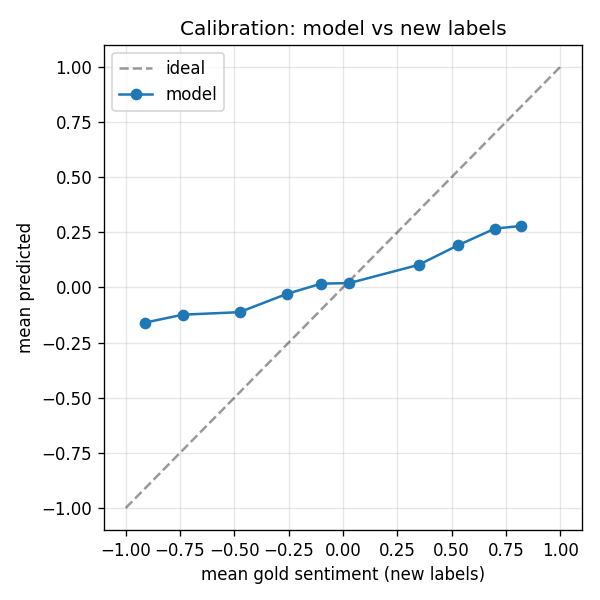
\includegraphics[width=0.5\linewidth]{outputs/eval_new_dataset/calibration.png}
\caption{Calibration of the v2.0 head against the decisive labels: mean prediction per label
decile. The slope well below one is the under-polarisation that the v2.1 loss was designed to
remove; on the v2.1 test split the prediction spread equals the label spread.}
\label{fig:calibration}
\end{figure}

\textbf{Cross-distribution check.} On the Sonnet holdout, which follows the older tone-based
scoring rule, v2.1 keeps most of v2.0's correlation (0.606 vs.\ 0.628), keeps a calibrated spread
(std ratio 1.02 vs.\ 0.73) and acquires a mild positive mean bias of $+0.06$. The head has learned
the decisive rule rather than overfitting the DeepSeek labeller's style, and a per-deployment
affine offset would remove the bias if absolute scores were consumed on a tone-labelled corpus.

\subsection{Tagging}

Table~\ref{tab:ner} breaks the v2.1 tagger down by type on the test split. Precision is high for
organisations and tickers and recall is low everywhere; dates and percentages are barely
recalled, but they carry no sentiment. Labelling a ticker only when the symbol appears literally makes TICKER spans rare,
so that row rests on 1{,}127 gold spans and should be read as an estimate with wide error bars;
it does not by itself explain why recall on those spans is low.

\begin{table}[H]
\centering\small
\begin{tabular}{@{}lrrrr@{}}
\toprule
\textbf{Type (v2.1, test split)} & Precision & Recall & F1 & Gold spans \\
\midrule
ORG & 0.885 & 0.564 & 0.689 & 34{,}464 \\
PERSON & 0.694 & 0.231 & 0.347 & 11{,}372 \\
TICKER & 0.861 & 0.148 & 0.253 & 1{,}127 \\
MONEY & 0.802 & 0.352 & 0.489 & 5{,}071 \\
PERCENT & 0.670 & 0.176 & 0.278 & 5{,}677 \\
DATE & 0.863 & 0.061 & 0.114 & 11{,}879 \\
\midrule
All types & 0.844 & 0.370 & 0.514 & 69{,}590 \\
\bottomrule
\end{tabular}
\caption{Span-level tagging by entity type, end to end with CLS-only global attention.}
\label{tab:ner}
\end{table}

\subsection{Error modes}

The audit of high-confidence disagreements characterised the residual errors as model
behaviours rather than label noise:
\begin{itemize}
  \item \textbf{Legal outcomes.} The model anchors on negative keywords (\emph{ban}, \emph{sue},
        \emph{probe}, \emph{antitrust}) even when the entity \emph{won}: ``Apple wins bid to
        pause Watch ban'' scored $-0.51$ against a label of $+0.5$.
  \item \textbf{Secondary and list-style mentions} in market wraps are under-read. About 3.7\% of
        all covered entities carry a strong label but receive a flat score; expressed as a share
        of the strongly labelled entities alone the rate is 21.3\% (Table~\ref{tab:v21}).
  \item \textbf{Charged context around an incidental entity} (a company named only as a benchmark
        or partner) is over-read.
  \item \textbf{Coverage.} Sentiment is produced only for the roughly half of entities the tagger
        finds; improving recall is the largest available gain and would also change the
        composition of every downstream aggregate.
\end{itemize}

\subsection{The scored corpus, illustrated}

Figure~\ref{fig:nvda} shows one ticker's monthly sentiment from the corpus scored for the market
study. The broad shape (a trough in the 2022 GPU downturn, a rise through the 2023--24 AI
build-out, softening in 2025) is plausible, but two features are data artefacts rather than
model outputs: the May~2023 dip sits on a week with no tier-1 coverage at all, and the sharp rise
in article counts in 2025 partly reflects a new wire source entering the tier-1 set. Monthly
aggregates at this granularity are noisy; the reviewers' recommendation to read them at daily
granularity around known events stands.

\begin{figure}[H]
\centering
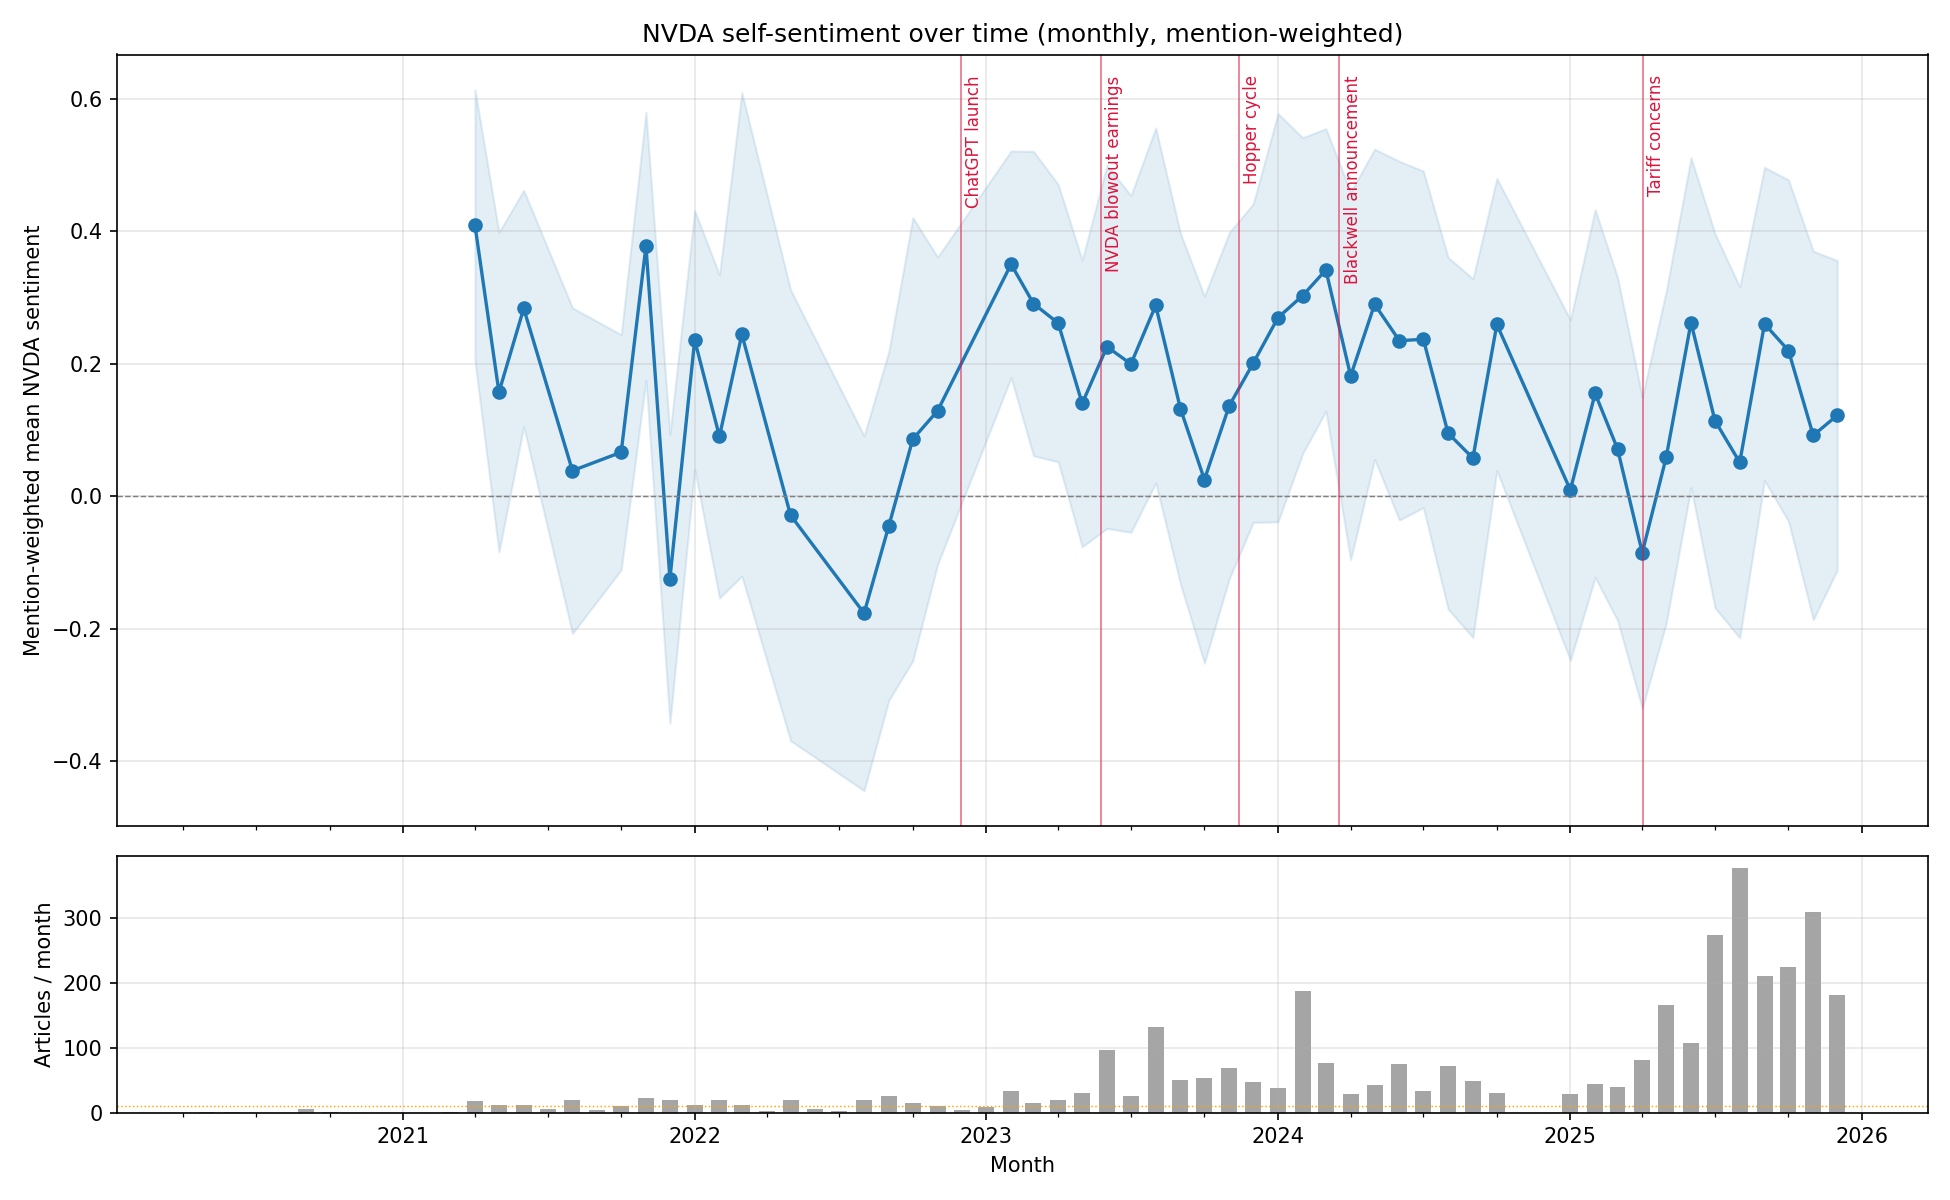
\includegraphics[width=0.92\linewidth]{outputs/inference/nvda_sentiment_timeseries.png}
\caption{Monthly mention-weighted NVIDIA sentiment (v2.0 scores over tier-1 articles) with
article counts. Months with fewer than ten articles are omitted.}
\label{fig:nvda}
\end{figure}

% =====================================================================
\section{Do the scores predict returns or volatility?}
\label{sec:signal}

\subsection{From article scores to a daily panel}

All tier-1 articles for the S\&P~500 universe were scored end to end with the v2.0 checkpoint
(118{,}033 unique articles, May--June 2026 inference run). Each article's entity records were
resolved to tickers with a constituent list plus a hand-made alias table and a blocklist of
non-companies (regulators, exchanges, news outlets), and the per-ticker score of an article is the
mention-weighted mean over the aliases that resolved to it. The daily signal \code{sent\_mw} for a
(ticker, date) pair is the mention-weighted mean over that day's articles. The date attached to
each article at inference time was the calendar date of its publication timestamp, taken as
written and with no conversion to New York time; articles whose date had no trading session, such
as weekend and holiday items, had no price bar to join to and were dropped from the panel. This
dating rule is what Section~\ref{sec:lookahead} shows to be wrong. The vendor-polarity baseline
used a different rule, rolling each article forward to the next available session.

The panel joins the signal to EODHD daily prices (open, close, adjusted close) and attaches
forward close-to-close returns at 1, 5 and 20 trading days, a size proxy (log dollar volume) and
1- and 12-month momentum controls. It has 60{,}888 ticker-days across 502 tickers from
23 March 2020 to 31 December 2025 (1{,}441 trading days) with a median of 45 names per day
(10th--90th percentile 8 to 64). The panel keeps thin days; each test applies its own floor, five
usable names for the information coefficient and the event study, ten for the quintile
portfolios. The universe is the current constituent list, which is a survivorship bias; for a
dollar-neutral long-short test it is second order, but it is not claimed away.

\subsection{The tests}

Five standard cross-sectional tests were run in sequence, each as its own script:
\begin{enumerate}
  \item \textbf{Information coefficient.} For each day, the Spearman rank correlation between
        the signal and the forward return across names; the daily series is summarised by its
        mean, its information ratio (mean over standard deviation), a Newey--West
        $t$-statistic \cite{newey1987} and the share of positive days.
  \item \textbf{Fama--MacBeth regressions} \cite{fama1973} of the forward return on the
        daily-standardised signal and the controls; the average slope is the return per one
        cross-sectional standard deviation of sentiment.
  \item \textbf{Event study.} Cumulative abnormal return (relative to the equal-weight universe)
        after top-quintile and bottom-quintile sentiment days, traced 20 sessions out.
  \item \textbf{Long-short backtest.} Daily quintile portfolios, long the top and short the
        bottom fifth, dollar-neutral, overlapping $H$-day holding, equal- and value-weighted,
        with two execution conventions: \emph{paper} entry at the signal day's close and
        \emph{tradable} entry at the next session's open; costs at 5 and 10\bps{} per side; the
        last 30\% of dates held out as a check.
  \item \textbf{Market-on-close feasibility audit.} Every article's publication timestamp
        converted to New York time and compared with a 15:45~ET cutoff for market-on-close orders,
        and the signal rebuilt on the first close by which each article was knowable. The
        committed script re-runs the one-day backtest and the day-one return decomposition on
        that corrected signal; the corrected information coefficient and the volatility test
        were computed separately and by hand, and the Fama--MacBeth and event-study tests were
        never re-run (Section~\ref{sec:open}).
\end{enumerate}
An article-level polarity score supplied with the news feed was run through the same backtest as
a baseline.

\subsection{First pass: an apparent success}
\label{sec:firstpass}

The first pass produced the numbers in Table~\ref{tab:firstpass}: a small but statistically
strong one-day IC that decays with horizon, a Fama--MacBeth slope of 10\bps{} per standard
deviation that survives the controls, and an event-study spread of $+36\bps$ on day one
(Figure~\ref{fig:event}). The backtest then split the picture: with paper close entry the
one-day strategy had a gross Sharpe ratio of 2.9, while the tradable next-open version was
\emph{negative} at every holding period (Table~\ref{tab:backtest}, Figure~\ref{fig:equity}).
The decomposition of the day-one spread explained why: of $+36\bps$ close to close, $+41\bps$
occurred in the overnight gap between the signal close and the next open, and $-5\bps$ in the
following session. The working conclusion at that point was ``genuinely predictive but
untradable''.

\begin{table}[H]
\centering\small
\begin{tabular}{@{}lrrrr@{}}
\toprule
\textbf{Horizon} & mean IC & IC IR & NW $t$ & days $>0$ \\
\midrule
1 day & $+0.0204$ & 0.097 & 3.65 & 54.7\% \\
5 days & $+0.0166$ & 0.080 & 2.92 & 53.8\% \\
20 days & $+0.0096$ & 0.045 & 1.48 & 53.7\% \\
\bottomrule
\end{tabular}
\caption{First-pass information coefficients on the naive panel. The Fama--MacBeth slopes of
\code{sent\_mw} on the same panel are $+10.3$, $+11.2$ and $+4.8\bps$ per standard deviation at
1, 5 and 20 days (Newey--West $t$ 6.70, 3.70 and 0.88). These numbers are contaminated by
look-ahead (Section~\ref{sec:lookahead}) and are shown for the record.}
\label{tab:firstpass}
\end{table}

\begin{figure}[H]
\centering
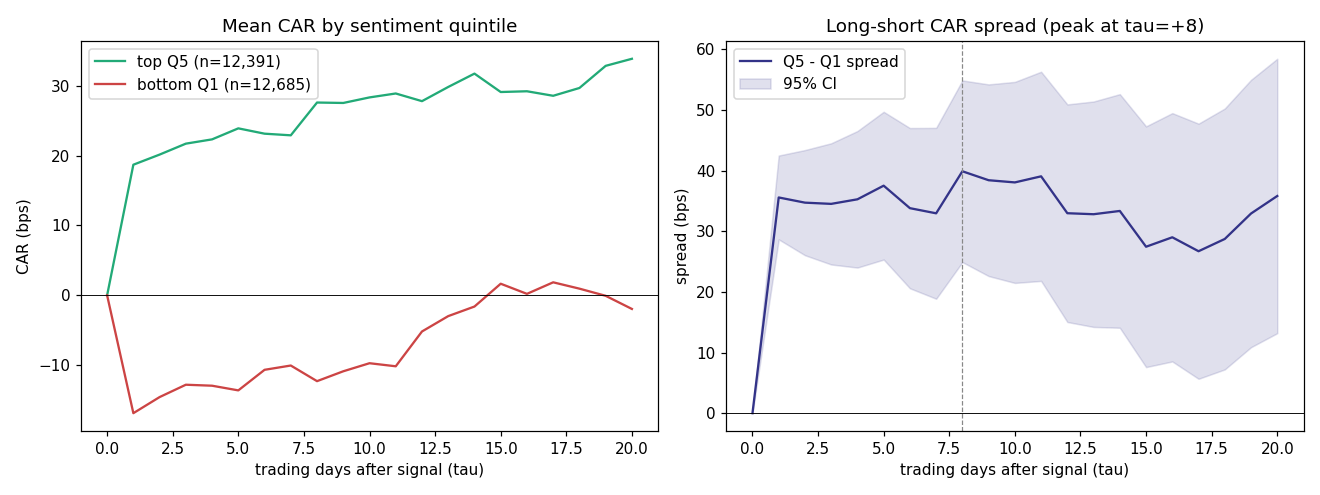
\includegraphics[width=\linewidth]{signal_strategy/outputs/event_study_car.png}
\caption{First-pass event study: mean cumulative abnormal return after top-quintile and
bottom-quintile sentiment days, and the long-minus-short spread with a 95\% band. The band treats
events as independent, which the reviewers rightly objected to; the day-one jump is the overnight
gap that turned out to be look-ahead.}
\label{fig:event}
\end{figure}

\begin{table}[H]
\centering\footnotesize
\setlength{\tabcolsep}{4pt}
\begin{tabular}{@{}rlrrrrr@{}}
\toprule
$H$ & entry & gross Sharpe & gross bps/day & net Sharpe @5\bps & net Sharpe @10\bps & turnover/yr \\
\midrule
1 & paper (signal close) & $+2.93$ & $+25.4$ & $+1.12$ & $-0.69$ & 395$\times$ \\
1 & tradable (next open) & $-0.72$ & $-4.5$ & $-3.22$ & $-5.70$ & 395$\times$ \\
5 & paper (signal close) & $+1.14$ & $+4.3$ & $+0.28$ & $-0.58$ & 82$\times$ \\
5 & tradable (next open) & $-0.48$ & $-1.7$ & $-1.41$ & $-2.33$ & 82$\times$ \\
8 & paper (signal close) & $+0.80$ & $+2.5$ & $+0.15$ & $-0.50$ & 51$\times$ \\
8 & tradable (next open) & $-0.41$ & $-1.2$ & $-1.09$ & $-1.77$ & 51$\times$ \\
\bottomrule
\end{tabular}
\caption{First-pass quintile long-short backtest, equal weight. Even the infeasible paper
version does not clear 10\bps{} of costs, because the edge is concentrated on day one and
requires about 400 portfolio turnovers a year.}
\label{tab:backtest}
\end{table}

\begin{figure}[!t]
\centering
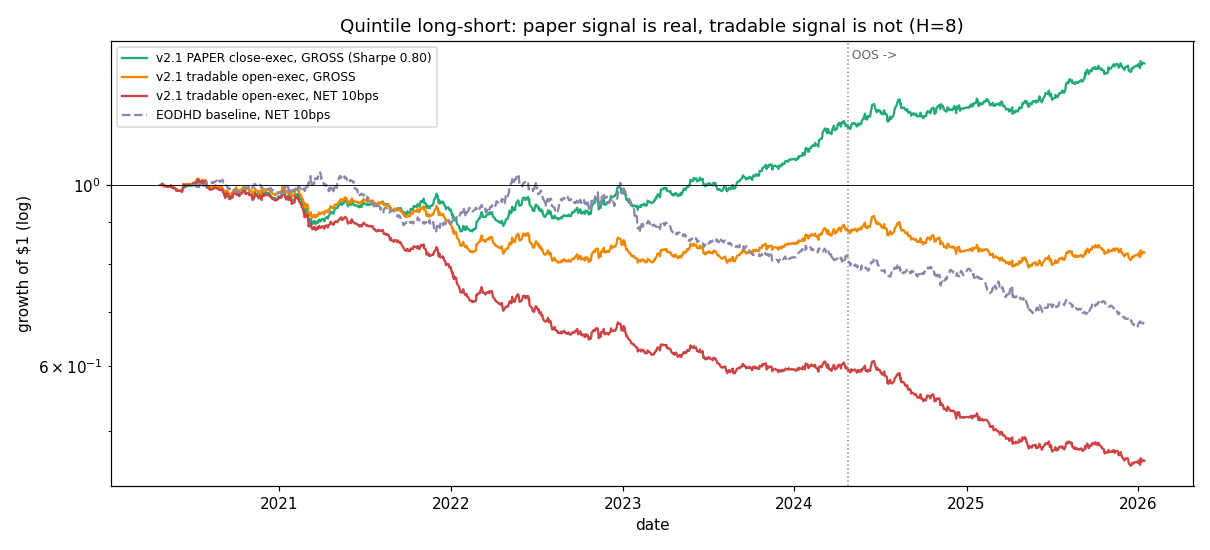
\includegraphics[width=\linewidth]{signal_strategy/outputs/ls_equity_curve.png}
\caption{First-pass equity curves for the eight-day holding period: paper close entry compounds
upward; tradable next-open entry, gross and net, drifts down, as does the vendor-polarity
baseline. The legend labels the signal ``v2.1''; the scores were produced by v2.0.}
\label{fig:equity}
\end{figure}

\subsection{The look-ahead, and the corrected results}
\label{sec:lookahead}

The question ``could we enter at the signal-day close with a market-on-close order?'' forced an
audit of \emph{when} each article was published relative to the session it had been assigned to.
About a quarter of the articles, including the 4--6~pm earnings-release spike, were not publicly
available by 15:45~ET on their assigned day. An earnings report published at 5~pm Monday carried
Monday's date, so the ``prediction'' compared Monday's close with Tuesday's close, a return that
contains the market's own reaction to the article. The model was not forecasting Tuesday; it was
reading Monday-evening news that Monday's close could not know and that Tuesday's open had already
priced. The same contamination inflates the IC, the Fama--MacBeth slopes and the event study, not
just the backtest.

Rebuilding the signal on the first close by which each article was knowable gives
Table~\ref{tab:feasible}. The IC is indistinguishable from zero at every horizon; the
implementable market-on-close strategy loses money; after-hours news traded at the next open is
also flat, and the feasible signal's own overnight gap is $+1.5\bps$ against $+40.9\bps$ before
the correction. News published during the session is in the price by the close, and after-hours
news is in the price by the open: the market absorbs this news faster than a daily-bar strategy
can act at any entry point the current machinery can express. One qualification belongs with the
table. The published late-news row assigns each article to its first feasible close and then
enters at the \emph{following} open, one session later than a trader could act; a reviewer ran
the correctly timed next-morning version and also found it flat, at $-4.9\bps$ from open to
close. Pre-market news traded at that same day's open was never tested at all
(Section~\ref{sec:open}).

\begin{table}[H]
\centering\small
\begin{tabular}{@{}lrrr@{}}
\toprule
\textbf{Horizon} & original IC (naive panel) & feasible IC & feasible NW $t$ \\
\midrule
1 day & $+0.0204$ ($t$ 3.65) & $-0.0067$ & $-1.39$ \\
5 days & $+0.0166$ ($t$ 2.92) & $-0.0020$ & $-0.39$ \\
20 days & $+0.0096$ ($t$ 1.48) & $+0.0025$ & $+0.41$ \\
\midrule
\multicolumn{2}{@{}l}{\textbf{Strategy variants, $H=1$, equal weight}} & gross Sharpe & gross bps/day \\
\multicolumn{2}{@{}l}{Original signal, close entry (look-ahead)} & $+2.93$ & $+25.4$ \\
\multicolumn{2}{@{}l}{Feasible signal, market-on-close, close to close (implementable)} & $-0.55$ & $-3.7$ \\
\multicolumn{2}{@{}l}{After-hours news only, next-open entry} & $-0.18$ & $-1.3$ \\
\bottomrule
\end{tabular}
\caption{Results after enforcing a 15:45~ET knowability cutoff. An independent recomputation
from the same corrected panel obtained a one-day IC of $-0.0006$ ($t$ $-0.10$); the verdict is
the same and the difference reflects that the correction was built ad hoc rather than as a
committed script (Section~\ref{sec:open}). The last row enters one session later than a trader
could act; see the text.}
\label{tab:feasible}
\end{table}

A second, sharper test by one reviewer simply dropped the ticker-days that the feasibility rule
reassigns and re-ran the IC on the rest: it fell from $+0.0204$ ($t$ 3.65) to $+0.0037$
($t$ 0.68). More than 80\% of the headline IC came from the after-hours quarter of the corpus.

The right reading of the strong first-pass numbers is therefore that the model measures well the
sentiment the market prices in. The entity-level signal also had a clearly stronger paper edge
than the vendor's article-level polarity, which suggests that the model adds cross-sectional
ranking value over an off-the-shelf score without establishing it: as one reviewer noted, that
comparison is look-ahead on both sides. What does not exist is a daily-bar opportunity to
trade it.

\subsection{Volatility: the result that survives}

Sentiment \emph{magnitude} carries information that direction does not. On the corrected panel,
$|\code{sent\_mw}|$ predicts the next day's absolute return with a cross-sectional rank IC of
$+0.024$ (Newey--West $t$ 5.3) after residualising on trailing 21-day realised volatility; on the
uncorrected panel, before the knowability correction, the raw figure was $+0.05$ to $+0.06$
($t\approx12$). A reviewer's replication added same-day absolute return as a further control and
still found $+0.019$ ($t$ 3.7), stable in every year from 2021 to 2025. Intense news tone today
means a bigger move tomorrow, direction unknown.

This is a promising non-directional candidate feature for a volatility or risk model, and both
the study and the replicating reviewer rated it the top surviving use. It is not
deployment-ready. It has no committed script, so the exact numbers are not reproducible from the
repository; and it has not been hardened with an earnings-day control, an
overnight-versus-intraday split of the predicted move, or a frozen out-of-sample period.

\subsection{External review}

The study was reviewed read-only by two independent model-based reviewers. The first diagnosed
the timing problem from the code and the first-pass write-up, before the corrected numbers
existed, and recommended withdrawing the claim of predictive content until the tests were
rebuilt point in time. The second read the already-corrected document, then independently
recomputed the diagnosis from the artefacts on disk and quantified it, and separately replicated
the volatility result with an extra control. The volatility test post-dates the first review, so
only one reviewer has confirmed it. The further weaknesses they identified, accepted rather than
silently fixed, are:
\begin{itemize}
  \item the event-study $t$-statistic of 10 treats thousands of overlapping same-day and same-ticker
        events as independent; portfolio-level inference with autocorrelation-robust errors is the
        right tool;
  \item the ``size'' control is same-day dollar volume, which is a liquidity measure and reacts to
        the news itself, so it is a post-treatment control;
  \item the holding period was chosen on the full sample, so the 70/30 date split is a report, not
        a true holdout;
  \item survivorship in the universe, silent zeros for missing price bars (worst in the short leg),
        an additive mixing of adjusted and unadjusted price bases in the decomposition, forced
        quintiles on thin cross-sections, and a fixed autocorrelation lag for 20-day overlapping
        returns;
  \item the ``after-hours news at the next open'' test entered one session too late; the correct
        next-morning test, run by the reviewer, is also flat ($-4.9\bps$ open to close);
  \item the corrected IC is significantly \emph{negative} in 2023 and 2024 ($t\approx-2$ each), a
        possible short-horizon reversal that is untested.
\end{itemize}
None of these change the sign of the conclusion, but they bound it: the honest claim is ``no
detected edge'', not ``an edge of exactly zero''.

\subsection{Open items}
\label{sec:open}

\begin{enumerate}
  \item Commit a script that rebuilds the knowability-corrected panel and re-runs the IC, the
        volatility test, Fama--MacBeth and the event study on it, so that the correction is
        reproducible. Only the one-day backtest and the return decomposition are currently
        reproducible from a committed script; the corrected IC and volatility numbers were
        computed by hand, and the Fama--MacBeth and event-study sections exist only in their
        contaminated form.
  \item Test pre-market news (05:00--09:00~ET, about 28\% of articles, knowable before the 9:30
        open) traded at the same day's open, the one daily-bar channel the current code cannot
        express.
  \item Check the 2023--24 negative-IC reversal hint with a proper short-horizon reversal test.
  \item Re-score the corpus with v2.1, whose head is better calibrated than v2.0's, and re-run
        the tests. Because the IC and quintile tests use ranks, the under-polarisation of v2.0
        matters less than it would for magnitude-based uses, but the volatility test does use
        magnitudes.
  \item Use point-in-time index membership.
\end{enumerate}

% =====================================================================
\section{Conclusions}
\label{sec:conclusions}

The model works as a reader: given a whole article, it scores what the news implies for each
named entity with a correlation of about 0.64 to LLM labels on unseen articles, with calibrated
magnitudes and strong performance on tickers. Its limits are equally clear: it finds only about
half of the entities, it can misread who won a dispute, and its tagger's CRF layer never trained.
The market tests are a negative result with a positive lesson. A signal that looked like a
Sharpe-2.9 strategy was an artefact of dating after-hours news to the session that had already
closed; once knowability is enforced, daily bars are too coarse to trade this news at any entry
point that was tested, and one channel, pre-market news at the same day's open, remains untested.
The honest claim is no detected edge rather than an edge of exactly zero. What remains is a good
measurement instrument, useful for attribution and monitoring and as a candidate volatility
feature, and a study whose corrections are documented in full so that the next pass starts from
the right place.

\bibliographystyle{plain}
\begin{thebibliography}{9}
\bibitem{beltagy2020longformer} I. Beltagy, M. E. Peters and A. Cohan. Longformer: The
  long-document transformer. \emph{arXiv:2004.05150}, 2020.
\bibitem{lin1989ccc} L. I-K. Lin. A concordance correlation coefficient to evaluate
  reproducibility. \emph{Biometrics} 45(1):255--268, 1989.
\bibitem{fama1973} E. F. Fama and J. D. MacBeth. Risk, return, and equilibrium: empirical tests.
  \emph{Journal of Political Economy} 81(3):607--636, 1973.
\bibitem{newey1987} W. K. Newey and K. D. West. A simple, positive semi-definite,
  heteroskedasticity and autocorrelation consistent covariance matrix. \emph{Econometrica}
  55(3):703--708, 1987.
\end{thebibliography}

\appendix
% =====================================================================
\section{The sentiment labelling prompts}
\label{app:prompts}

The two prompts below produced the decisive label set (Table~\ref{tab:labels}). The first was
given to DeepSeek v4-flash as the system prompt for every article; the second was given to Kimi,
with the article and the list of already-extracted PERSON entities, to re-score every person. They
are reproduced verbatim from \code{data\_label\_criteria/} except that a few non-ASCII symbols
(arrows, a star, currency signs, typographic quotes and dashes) are replaced by ASCII equivalents
for typesetting. The earlier Sonnet prompt used for the v2.0 labels differs most consequentially
in its sentiment section: it scored the article's tone toward the entity and defined 0.0 as
``factual mention'', without the implication rule or the adversarial examples. The decisive prompt
also tightened the extraction rules, separating proper-name mentions from descriptive epithets
and creating a ticker record only when the symbol appears literally.

\subsection{Entity and sentiment labelling prompt (v2.2, decisive)}
\lstinputlisting{report_assets/prompt_decisive.txt}

\subsection{PERSON re-scoring prompt}
\lstinputlisting{report_assets/prompt_person.txt}

\clearpage
% =====================================================================
\section{What the public repository contains}
\label{app:repo}

The repository at \url{https://github.com/Russell-Ding/entity_sentiment_model_pipeline} holds the
code needed to understand and audit the results in this report. Table~\ref{tab:repo} lists it.
Not included, by design: the news and price data (EODHD terms), the label files (derived from
that data), the model weights (1.8\,GB per version), the inference outputs and panels derived from
the news data, and the data-collection, labelling and model-training code. The label
specification and prompts, the model cards with their evaluation metrics, and the evaluation and
signal-study code are all present, so each table in this report can be traced either to the
script that produced it or to the metric file it was read from. The exceptions are the corrected
information coefficient and the volatility result of Section~\ref{sec:signal}, which were
computed by hand and have no committed script (Section~\ref{sec:open}).

\begin{table}[H]
\centering\footnotesize
\begin{tabularx}{\linewidth}{@{}P{5.9cm}Y@{}}
\toprule
\textbf{Path} & \textbf{Contents} \\
\midrule
\code{docs/project\_report.tex}, \code{.pdf} & this report and its source \\
\code{docs/report\_assets/} & the two labelling prompts of Appendix~\ref{app:prompts} as ASCII
  text, included by the report source \\
\code{models/} & the model: Longformer wrapper, CRF NER head, cross-attention sentiment head with
  both loss modes, the pipeline class that combines them (Section~\ref{sec:model}) \\
\code{training/preprocessing.py}, \code{dataset.py}, \code{metrics.py} & label schema (the 15 BIO
  tags, sentiment-bearing types), mention-to-token alignment, batching, and the metric functions
  used by the evaluations; the training loop itself is withheld \\
\code{scripts/evaluation/} & end-to-end evaluation (raw text to scored entities, IoU matching,
  coverage), gold-mask evaluation, calibration baseline, gap analysis, arm comparison,
  cross-distribution comparison on the Sonnet holdout, disagreement audit
  (Section~\ref{sec:validation}) \\
\code{scripts/inference/} & batch scoring of a news file with a checkpoint (default v2.0) \\
\code{scripts/postprocessing/} & ticker resolution, per-article and daily ticker sentiment,
  leakage-safe return mapping, time-series plot \\
\code{scripts/analysis/inspect\_ner\_head.py} & reproduces the CRF measurements of
  Section~\ref{sec:crf} \\
\code{signal\_strategy/src/} & panel construction, IC, Fama--MacBeth, event study, long-short
  backtest, market-on-close feasibility, runner (Section~\ref{sec:signal}) \\
\code{signal\_strategy/outputs/} & metric JSON files, daily IC series and plots of the study \\
\code{signal\_strategy/RESULTS.md}, \code{CONSOLIDATED\_REPORT.md} (and their PDFs),
  \code{README.md}, \code{notes/reviews/}, \code{research/} & the study's working documents in
  original form with a correction note, the two raw external reviews and the review prompt, the
  literature review \\
\code{trained\_model/v*/} & model cards, architecture configs and end-to-end evaluation metrics for
  v1.0, v2.0 and v2.1 \\
\code{outputs/} & evaluation summaries, calibration figure and gap analysis, the label-noise
  audit, corpus-coverage investigations and the NVIDIA time series \\
\code{data\_label\_criteria/} & the labelling specification and the three prompts \\
\code{data/reference/} & the alias table and non-company blocklist used for ticker resolution \\
\code{notebooks/} & Colab launchers for inference and the two evaluations (outputs stripped) \\
\code{README.md}, \code{CLAUDE.md}, \code{LICENSE},
  \code{requirements.txt} & repository front door, working notes for agents, MIT licence with its
  data and weights exclusion, dependencies \\
\bottomrule
\end{tabularx}
\caption{Public repository map.}
\label{tab:repo}
\end{table}

\end{document}
